\section{State of the art in ESD testing}
\label{sec:state-art-esd-testing}

Electronic hardware robustness is tested against electrostatic discharges using different test methods and standards.
Each method reproduces a specific discharge event \gls{esd} in laboratory conditions.
In this chapter, relevant \gls{esd} generators for this research work are detailed.

In ESD testing, a distinction is often made between so-called system-level level tests and \gls{ic} level tests.
System-level tests reproduce discharge events encountered by a system deployed in the field.
Silicon-level tests target \gls{esd} events happening during \gls{ic} manufactoring.

System-level tests involve higher voltage and current amplitudes, and are more harmful for electronic devices than \gls{ic} level tests.

\subsection{Transmission Line Pulsing (TLP)}

% tlp concept
\gls{tlp} generators generate a fast rectangular pulse.
The pulse is produced by the discharge of a coaxial cable (Fig. \ref{tlp_concept}).
The cable is charged by a high-voltage power supply then discharged into a load by switching a relay.
The charge is performed through a high value resistor to keep the current small and avoid oscillations on the cable.

\begin{figure}[!h]
  \centering
  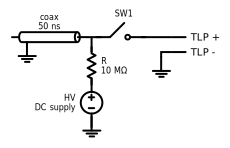
\includegraphics[width=\textwidth]{src/1/figures/tlp_concept.pdf}
  \caption{Minimal example of a \gls{tlp} system}
  \label{tlp_concept}
\end{figure}

% advantages of tlp systems
TLP systems constitute very well-controlled test generators where the pulse is generated inside a shielded and isolated environment.
Characteristic impedance can be controlled up to the load.
Those features allow for extremely clean and repeatable pulse waveforms.
The main characteristics of a TLP waveform are given in figure \ref{tlp_pulse}

\begin{figure}[!h]
  \centering
  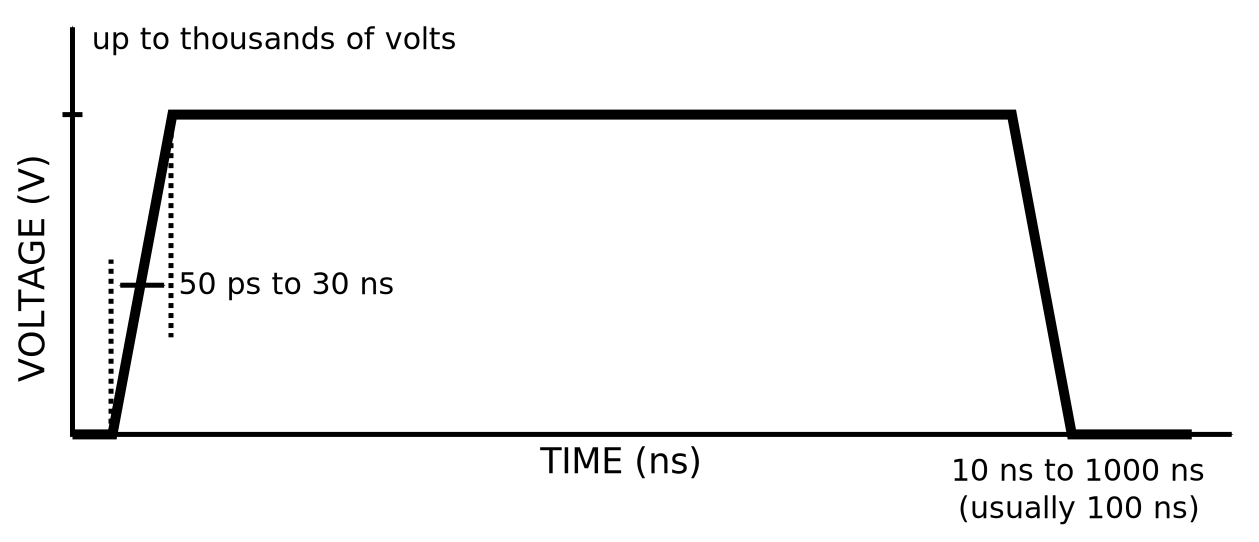
\includegraphics[width=\textwidth]{src/1/figures/tlp_pulse.pdf}
  \caption{Main characteristics of a \gls{tlp} pulse on a resistive load}
  \label{tlp_pulse}
\end{figure}

% principle of tlp for i(v) curve extraction
Using time-domain reflectometry, it is possible to reconstitute the current and voltage waveforms inside the load,
from measured current and voltage inside the \gls{tlp} \cite{TLP}.
The superposition of the incident and reflected pulses during the discharge show that the voltage and current
measured inside the generator are direct image of the ones accross and through the load.

\gls{tlp} are extensively used for characterizing the response of ESD protections \cite{TLPforESDProtectionCz}
or testing the response of systems and devices against a clean and well repeatable pulse \cite{TLPthroubleshooting, LacrampeTransientImmunity}.

%TODO: Detail more quasi-static characterization ?
%TODO: Example snapback/no snapback I(V) curve ?

\subsection{ESD Gun (IEC 61000-4-2 / ISO 10605)}

% What is the goal of this test
IEC 61000-4-2 and ISO 10605 standards define a system-level test waveform and test generator to reproduce the discharge of a human body through an electronic device.
This test is used very extensively for the qualification of products.

\begin{figure}[!h]
  \centering
  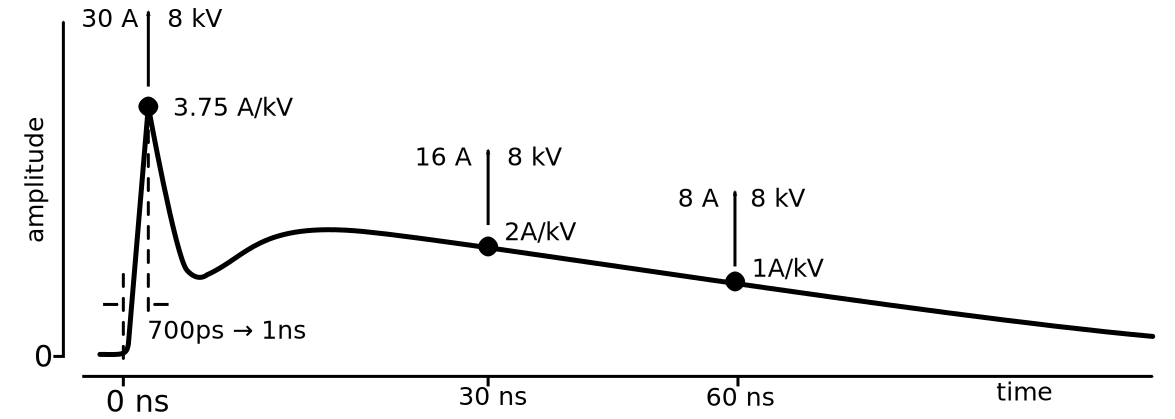
\includegraphics[width=\textwidth]{src/1/figures/iec61000-4-2_waveform.pdf}
  \caption{Main properties of an IEC 61000-4-2 pulse on a 2\textOmega\ resistive load}
  \label{iec_pulse}
\end{figure}

% How is the pulse generated
The generation of the ESD pulse is done by a resistor-capacitor discharge network.
The RC network alone though does not suffice to reproduce the waveform given in Fig. \ref{iec_pulse}.
Parasitic devices play an important part in shaping the waveform.

% Where does this standard applies
Each standard defines the construction and waveform requirements for this ESD generator, but with different fields of application.
IEC 61000-4-2\cite{iec61000-4-2} standard targets consumer electronics.
ISO 10605\cite{iso10605} standard is intented for automotive equipment.
The latter defines additional pulse waveforms to cover a wider range of ESD events (See fig \ref{iso_pulse}).

\begin{figure}[!h]
  \centering
  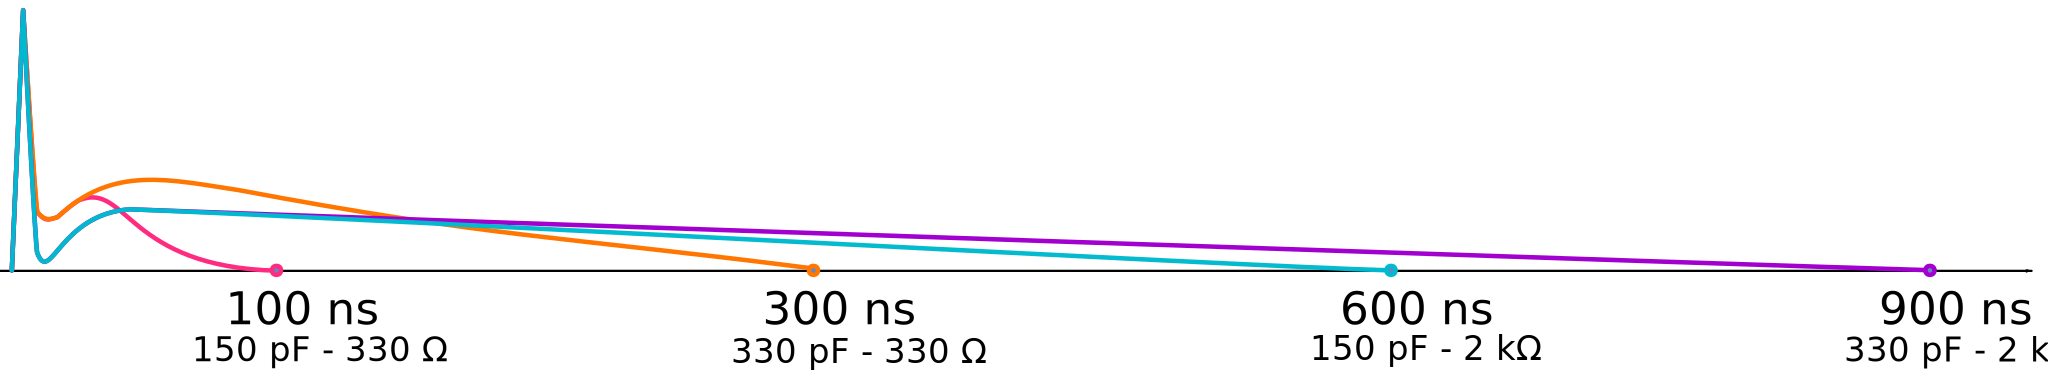
\includegraphics[width=\textwidth]{src/1/figures/iso10605_waveform.pdf}
  \caption{Waveforms defined in ISO 10605 standard on a 2\textOmega{} resistive load}
  \label{iso_pulse}
\end{figure}

%TODO: Annex F ISO 10605

\subsection{ISO 7637-2}

% Where does this standard applies
ISO 7637-2\cite{iso7637-2} is an automotive standard for testing immunity of electronic devices against transient electrical disturbances.
It is mostly targeting disturbances applied on supply lines.
This standard defines several waveforms.
Among them, pulses 2A and 3B are the closest to an electrostatic discharge.

% Pulse 2A - What is the goal of this pulse
Pulse 2A simulates the sudden disconnection of a load placed in parallel with the \gls{dut}.
In a car, it reproduces the switching of devices separated by inductive wiring harnesses.
When a load is abruptly switched off, the inductance opposes to the sudden interruption of current.
Instead of flowing through the load, the current is maintained and reported onto the \gls{dut} which can be damaged or disturbed in the process.
These events can be quite harmful with peak voltages above 50V during 50\textmu{}s.
This pulse can be an interesting testing waveform in the context of this entire document.
The characteristics of pulse 2A are given in fig. \ref{fig:iso_2a_pulse}.

\begin{figure}[!h]
  \centering
  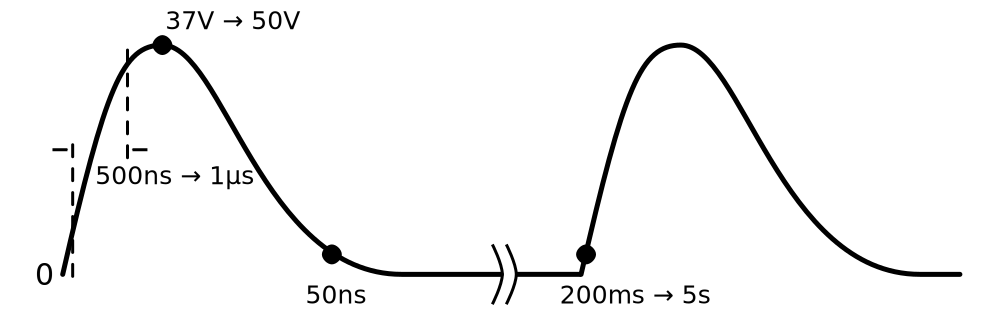
\includegraphics[width=0.7\textwidth]{src/1/figures/iso7637-2-2a.pdf}
  \caption{Waveform 2A defined in ISO 7637-2 standard on a 2\textOmega{} resistive load}
  \label{fig:iso_2a_pulse}
\end{figure}

% How is the pulse generated
ISO 7637-2 compliant stress generators are often implemented with R-C discharge networks.
It is the easiest way to produce the standardized waveform on a 2\textOmega{} resistor.
By construction, it is not the best way to reproduce the inductive behavior of the wiring harness.
However, it is a common method in the \gls{esd} field to define pulses on simple loads to make the manufacturing, testing and investigation more approachable.

% Pulse 3B - What is the goal of this pulse
Pulse 3B also simulates the result of a switching process on a wiring harness, causing negative spikes on a \gls{dut}.
Its waveform is given in fig. \ref{fig:iso_2b_pulse}.
Compared to pulse 2a, this waveform has a shorter duration and risetime and a higher amplitude.
Interestingly, it is one of the rare \gls{esd} waveforms to be defined on a 50\textOmega{} load.

\begin{figure}[!h]
  \centering
  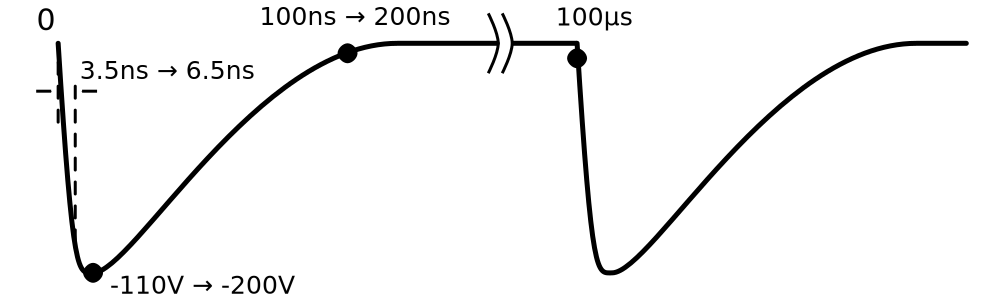
\includegraphics[width=0.7\textwidth]{src/1/figures/iso7637-2-3b.pdf}
  \caption{Waveform 3B defined in ISO 7637-2 standard on a 50\textOmega{} resistive load}
  \label{fig:iso_2b_pulse}
\end{figure}

\subsection{IEC 61000-4-4}

% Where does this standard applies - scope
The IEC 61000-4-4 standard \cite{iec61000-4-4}, also called burst test, defines a fast transient burst waveform for \gls{esd} testing.
It tests the immunity of electronic devices to repetitive fast transients on supply, signal and control ports.

% What is the pulse
The defined waveform is a double exponential pulse \ref{fig:iec_4_4_pulse} with a width of 50ns at 50\% of the peak amplitude.
It is defined for a 50\textOmega{} load, with a pulse period of 15ms and a burst period of 300ms.

\begin{figure}[!h]
  \centering
  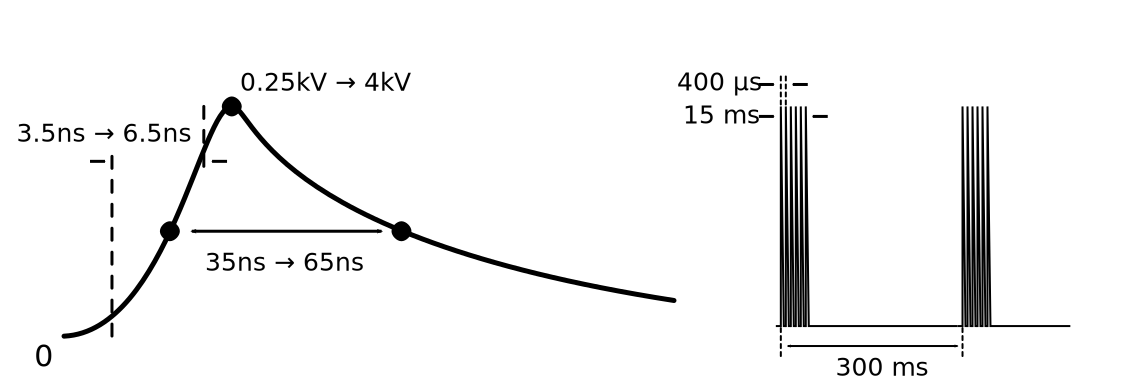
\includegraphics[width=\textwidth]{src/1/figures/iec61000-4-4_waveform.pdf}
  \caption{IEC 61000-4-4 waveform on a 50\textOmega{} resistive load}
  \label{fig:iec_4_4_pulse}
\end{figure}

% How is the pulse generated
The standard defines a circuit diagram for the generator, based on a resistor-capacitor network and spark-gap (Fig \ref{fig:iec_4_4_generator}).
The generator's output is a coaxial plug to prevent radiated emission during the discharge.

\begin{figure}[!h]
  \centering
  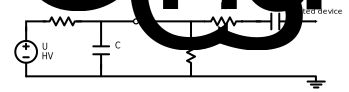
\includegraphics[width=\textwidth]{src/1/figures/iec61000-4-4_diagram.pdf}
  \caption{IEC 61000-4-4 generator circuit diagram}
  \label{fig:iec_4_4_generator}
\end{figure}

% Injection method - capacitive coupling clamp
This standard defines an injection method for powered lines called a \texit{capacitive coupling clamp} (Fig. \ref{fig:iec_4_4_clamp}).
This device is very relevant for this research work because injecting \gls{esd} onto powered devices and supplies in particular with good repeatability is rather challenging.
The device works by placing two large metallic plates in parallel, injecting the discharge on one of the plates and the wires inside a metallic tunnel connected to the other plate.

\begin{figure}[!h]
  \centering
  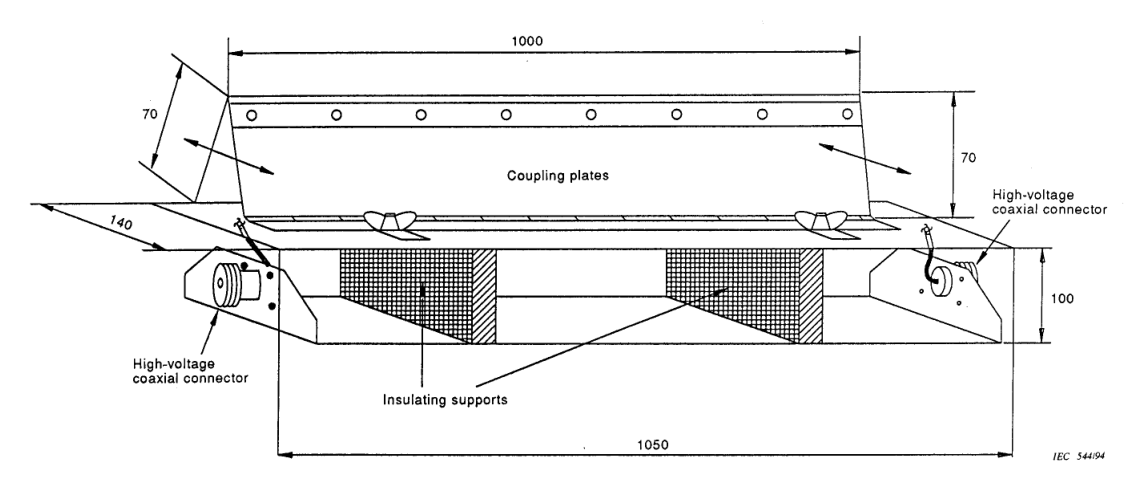
\includegraphics[width=0.8\textwidth]{src/1/figures/iec61000-4-4_clamp.png}
  \caption{IEC 61000-4-4 capacitive coupling clamp}
  \label{fig:iec_4_4_clamp}
\end{figure}

\subsection{IEC 62215 standard}

% Where does this standard applies - scope
The IEC 62215 standard \cite{iec62215} defines a method for measuring the immunity of an integrated circuit to conducted electrical transient disturbances.
This standard specifically targets testing of integrated circuits in operation, and as such is extremely relevant for this document.
In itself, the standard does not define a new test waveform.
It specifies to employ waveforms in ISO 7637-2 \cite{iso7637-2} for automotive devices and IEC 61000-4-4 \cite{iec61000-4-4} or IEC 61000-4-5 for industrial and consumer applications.
It focuses on understanding interactions between a conducted disturbance and performance degradation induced in integrated circuits.
The test method is quite similar to \gls{dpi} defined in IEC 62132-4 \cite{iec62132-4}.
The \gls{dpi} standard focuses on frequency domain immunity, while this standard tests time-domain immunity.

% How is the pulse generated
Disturbances are applied to the \gls{ic} pins via a coupling network.
A typical pin injection setup is given in Fig. \ref{fig:iec62215_setup}.

\begin{figure}[!h]
  \centering
  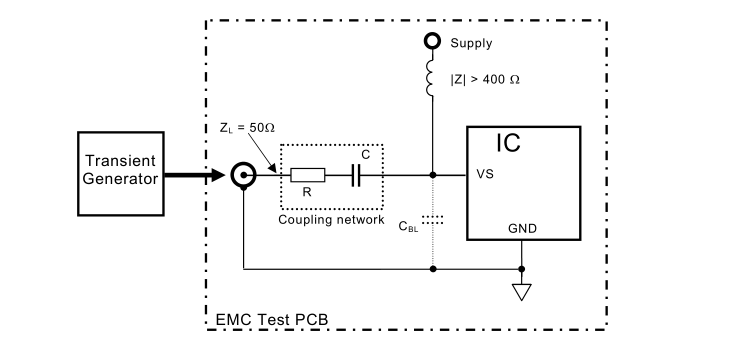
\includegraphics[width=0.9\textwidth]{src/1/figures/iec62215_setup.png}
  \caption{Typical injection setup via a coupling network}
  \label{fig:iec62215_setup}
\end{figure}

% Talk about immunity classes
Beyond test setup and waveforms, the standard defines immunity classes to categorize the behavior of integrated circuits exposed to disturbances during normal operation.
Classes range from A to E, with A describing the most robust devices in terms of functionnality.
In class A\textsubscript{IC}, the \gls{ic} performs within the defined tolerances during and after exposure to disturbance.
In class D\textsubscript{IC}, at least one monitored function of the IC does not perform within the defined tolerances during exposure and does not return to normal operation by itself, requiring an external intervention such as power reset.
In class E\textsubscript{IC}, at least one monitored function does not perform within the defined tolerances after exposure and can not be returned to proper operation.
